\cleardoublepage
\newrefsection
\chapter{文献综述}

\section{背景介绍}

随着Spectre\cite{kocher2020spectre}、Meltdown\cite{horn2018meltdown}等瞬态执行漏洞的提出,瞬态执行漏洞已经成为了现代处理器的关键漏洞。为了可以能在处理器 RTL 开发阶段尽早地发现并修复瞬态执行漏洞,处理器 Fuzzing 技术被用于处理器瞬态执行漏洞的挖掘。而在学术界,针对瞬态执行漏洞的处理器 Fuzzing 技术的研究一般基于开源的 RISCV 处理器进行,因而在这一章我们将对 RISC-V 指令集架构、瞬态执行攻击和处理器 Fuzzing 技术进行简单介绍。

\subsection{RISC-V指令集架构}
RISC-V 指令集架构(ISA)是一种开源的精简指令集架构。它由一个基本的整数指令 集和一组可选的指令集扩展组成。标准扩展包含整数乘除法扩展(M)、内存原子操作扩展(A)、单精度浮点扩展(F)、双精度浮点扩展(D)和压缩指令扩展(C)等。此外,控制和状态寄存器指令扩展(ZICSR)提供特权态管理功能, 而屏障指令扩展(ZIFENCEI)提供指令内存同步功能。\par

\begin{figure}[!h]
    \centering
    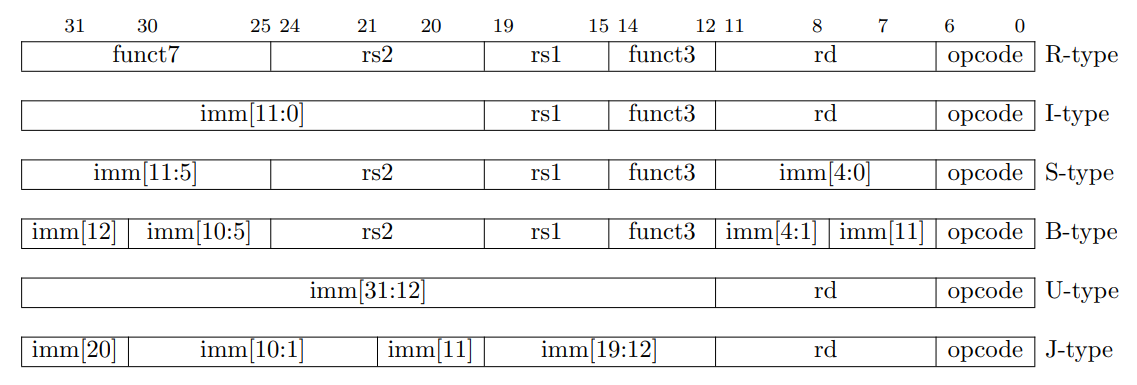
\includegraphics[width=\linewidth]{figure/proposal/riscv-base-instruct-format.png}
    \caption{RISCV基本指令格式}
    \label{review:base-inst}
\end{figure}
\begin{figure}[!h]
    \centering
    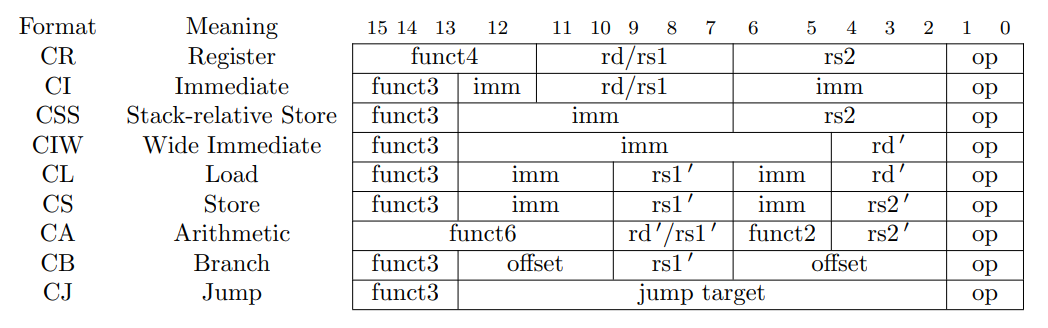
\includegraphics[width=\linewidth]{figure/proposal/riscv-compress-instruct-format.png}
    \caption{RISCV压缩指令格式}
    \label{review:compress-inst}
\end{figure}

RISC-V 指令分为 32 位常规指令和 16 位的压缩指令两种。 图\ref{review:base-inst}和图\ref{review:compress-inst}显示了所有 15 种指令类型的格式,每种指令由多个字段组成。32 位指令的指令格式由 opcode 字段决定,而 16 位指令的格式由 op 和 funct 字段同时决定。\par

指令字段可分为两类:\par

第一类是操作码相关字段,如 funct 和 opcode 字段。opcode 字段和 op 字段的低 2 位用于确定指令的长度,而 funct 字段和 opcode 字段的其它位用于确定指令的功能。通常,具有相似功能的指令有相同的 opcode 字段,并通过 funct 字段来区分。\par

第二类是操作数相关的字段,包括 imm,rs 和 rd 字段。其中 rs 字段用于选择源寄存器,imm 字段用于表示立即数,rd 字段用于选择目的寄存器,即写回指令结果的寄存器。\par

\subsection{瞬态执行攻击}
瞬态执行漏洞是现代处理器的关键漏洞。现代处理器为了追求高性能,广泛采用乱序执行和投机执行等技术提高硬件利用率。由于异常延迟处理和推测错误等原因,部分指令会被错误执行,虽然其执行结果会在后续被撤销,并不会影响处理器执行结果的正确性,但仍可能引起处理器微架构的状态变化。攻击者可以通过侧信道跟踪微架构的状态变化,进而恢复出处理器内部的机密信息,这种攻击方式称为瞬态执行攻击。\par

瞬态执行攻击过程包括三个子过程:\par

1.操纵控制流和数据流,人为创造异常延迟处理或者推测错误等场景,触发瞬态执行窗口。例如Meltdown 类型利用了延迟的权限检查,如对页表条目中的标志位的检查\cite{horn2018meltdown},或对浮点寄存器权限的检查\cite{stecklina1806lazyfp};而 Ret2spec\cite{maisuradze2018ret2spec}则通过毒害返回地址堆栈,引发返回地址的预测错误。\par

2.利用瞬态窗口绕过软件、硬件对安全边界的检查,访问秘密数据。例如幽灵式攻击通过对预测器的训练触发瞬态执行,通过暂时性改变控制流来绕过软件执行的安全检查;崩溃类型则利用异常延迟处理,赶在硬件原语完成执行的安全检查之前,完成对秘密数据的非法访问。\par

3.通过微体系结构的侧通道进行机密数据的泄露,已知的瞬态执行漏洞往往通过缓存\cite{yarom2014flush+}、分支预测器\cite{evtyushkin2018branchscope}、执行端口\cite{bhattacharyya2019smotherspectre}等时间侧信道进行信息泄露,但随着 cpu 复杂度的不断提高和瞬态攻击研究的不断推进,更多侧信道正在被发掘。\par

\subsection{处理器 Fuzzing}

Fuzzing 一种自动化的测试技术,它会根据一定的规则自动或者半自动地生成随机数据,然后输入到动态运行的被测程序入口,通过监控被测程序是否有异常情况发生(如系统崩溃,断言失败等)来发现存在的软件缺陷。同时一些 Fuzzing 生成器会根据被测程序插桩的信息反馈,有指向性的对输入数据进行突变,进一步提高异常触发的效率和提高程序测试的覆盖率。随着处理器复杂程度的提高,传统的处理器验证方式效果开始不断受限,研究人员转而将 Fuzzing 技术引入到处理器正确性验证领域 \cite{bruns2022efficient}\cite{canakci2021directfuzz}\cite{hur2021difuzzrtl}。\par

处理器 Fuzzing 和软件 Fuzzing 一样也由三个阶段组成:\par

1.在输入生成阶段,模糊器使用种子生成指令流,并根据前一轮的覆盖范围对指令流进行突变,如 DifuzzRTL\cite{hur2021difuzzrtl}使用静态分析技术生成指令,而 Huzz\cite{kande2022thehuzz} 则使用最优权重优化算法进行突变。\par

2.在硬件仿真阶段,Fuzzing 工具使用硬件插桩技术来收集当前输入的覆盖率,现有的 Fuzzing 工具设计了多种覆盖度量,诸如 mux 覆盖\cite{laeufer2018rfuzz}、控制寄存器覆盖\cite{hur2021difuzzrtl}和硬件行为覆盖\cite{kande2022thehuzz} 等。\par

3.在状态验证阶段,Fuzzing 工具提取 DUT 的架构状态,然后将其与参考模型(例如,ISA 模拟器)进行比较,其中不匹配的行为将被标记为 bug。

\section{国内外研究现状}

瞬态指令漏洞的 Fuzzing 检测作为处理器 Fuzzing 的变体,可以类似的分为输入生成阶段、测试执行阶段和漏洞检测阶段三部分。本章节将从这三个方面分别进行研究方向和研究进展的介绍。

\subsection{研究方向及进展}

\subsubsection{输入生成}
输入生成阶段负责生成尝试触发瞬态执行漏洞的测试程序。早期的硬件 Fuzzing 工具如 DifuzzRTL\cite{hur2021difuzzrtl}、TheHuzz\cite{kande2022thehuzz}等基本采用纯随机的方式进行测试指令的生成,处理器漏洞挖掘效率相对较低。为了进一步提高测试程序的质量,Razzle\cite{razzle}、Cascade\cite{soltcascade}等工具会对程序的控制流进行约束,以此提高程序执行的覆盖率;SpecDoctor\cite{hur2022specdoctor}等工作对指令的数据流进行了约束,通过提高相邻指令的数据依赖,提高其在处理器微架构执行时的难度。\par

为了充分利用瞬态执行漏洞的语义特点,一些测试程序生成工具采用基于模板突变的方法,试图高效的产生瞬态执行漏洞的变体。如Transynther\cite{moghimi2020medusa}是专注于 MDS 变体生成的工具,它使用已知的MDS构建块和微代码进行组合,来构造新的 MDS 泄漏,而SpeechMiner \cite{xiao2019speechminer}则专注于 Meltdown 变体的生成。但这种方法可能会导致漏洞同质化,缺乏挖掘全新漏洞的能力。\par

\subsubsection{测试执行}

测试执行阶段负责让后端处理器执行前端生成的测试程序,尝试在执行中触发瞬态执行漏洞。早期的工作会直接使用真实的处理器硬件执行测试程序,但是随着RTL漏洞检测重要性的提高,基于RTL仿真的瞬态漏洞测试执行工作,如IntroSpectre\cite{ghaniyoun2021introspectre}、SpecDoctor\cite{hur2022specdoctor}等开始兴起。Verilator\cite{snyder2013verilator}等开源工具为RTL仿真提供了条件,且在仿真的场景下还可以进行硬件插桩,便于后续阶段的漏洞检测。\par

但为了提高测试执行的效率,一些工作如Revixor\cite{oleksenko2022revizor}、Scam-V\cite{nemati2020validation}、Speculation at Fault\cite{hofmann2023speculation}等会对处理器硬件建立形式化模型,然后基于形式化模型进行测试执行,其中Revixor\cite{oleksenko2022revizor}支持 x86 指令,Scam-V\cite{hofmann2023speculation}支持 arm 指令,Speculation at Fault\cite{hofmann2023speculation}则是对Revixor\cite{oleksenko2022revizor}在异常相关类型漏洞上的一个补充。此外基于模型的测试方式也可以对模型直接进行瞬态执行漏洞的静态分析,如UPEC\cite{fadiheh2020formal}根据开源RTL手动建立有界模型,然后利用静态分析的技术寻找瞬态漏洞。

\subsubsection{漏洞检测}

漏洞检测阶段负责对测试执行的结果进行分析,进而判断是否触发了瞬态执行漏洞。差分测试是广泛使用的瞬态执行漏洞检测的方法,Revixor\cite{oleksenko2022revizor}、Speculation at Fault\cite{hofmann2023speculation}等工作都使用差分测试进行瞬态执行漏洞检测,
SpecDoctor\cite{hur2022specdoctor}更是在两个不同的阶段分别运用了差分测试。\par

此外还可以用基于约束的方法进行瞬态执行漏洞的检测,如Transynther\cite{moghimi2020medusa}、IntroSpectre\cite{ghaniyoun2021introspectre}通过检查缓冲区执行前后的变化进行漏洞检查,SpeechMiner\cite{xiao2019speechminer}通过测量竞争条件判断漏洞的可用性。\par

差分测试和约束判断的漏洞检测方法有时还需要硬件插桩的辅助。如果拥有 RTL 的源码,就可以通过 RTL 硬件插桩的方法为检测程序得到处理器内部的状态信息和事件信息,甚至可以在处理器内存内嵌约束判断的电路逻辑,在测试执行的同时直接进行漏洞约束的判断。

\subsection{瞬态执行漏洞 Fuzzing 存在的困难}

虽然软件 Fuzzing 技术已经十分成熟,并且硬件处理器 Fuzzing 框架也在逐渐完善,但是瞬态攻击漏洞的检测不同于普通的功能性检测,它的触发条件更加复杂、隐蔽、多样化,这使得现有的瞬态漏洞 Fuzzing 工作仍然存在很多不足。

\subsubsection{多样化的威胁模型和上下文}

瞬态执行漏洞可以在各种威胁模型和上下文设置\cite{kocher2020spectre}\cite{horn2018meltdown}\cite{ragab2021rage}\cite{van2006cacheout}中被执行。因为瞬态执行漏洞利用最底层的硬件特性发动攻击,所以任何运行在 CPU 上的实体(无论用户程序还是内核程序)都有可能成为攻击者或者受害者。且瞬态漏洞既可以从攻击者一方发动攻击(如 Meltdown),也可以从受害者一方发动攻击(如 Spectre)。此外各类 CPU 设置,诸如页表设置\cite{horn2018meltdown}、特权寄存器设置、飞地设置\cite{van2018foreshadow}、缓冲区设置\cite{moghimi2020medusa}等也会影响瞬态执行漏洞的执行。传统的模糊测试主要关注于如何扩展输入的覆盖率,其威胁模型和设置往往是单一且固定的;而瞬态执行漏洞的模糊测试框架则应尽量囊括各类可能的情况,因此在生成测试程序时需要充分考虑包括威胁模型、内存设置、瞬态执行的上下文在等众多配置。

\subsubsection{瞬态漏洞 Fuzzing 的指令生成}

基于模板的 Fuzzing 指令生成从已有的瞬态攻击模板出发进行突变,虽然可以快速找到某类瞬态执行攻击的变种,但是也被模板本身所局限,例如 Transynther\cite{moghimi2020medusa}专注于 MDS 变体生成、SpeechMiner \cite{xiao2019speechminer}专注于 Meltdown 变体的生成,故而不容易挖掘出新的瞬态漏洞。\par
另一些工作\cite{oleksenko2022revizor}则用随机的方法生成测试程序,这虽然可以摆脱突变模板的局限,但是因为瞬态漏洞触发的复杂性,这种抛弃了瞬态漏洞本身程序特点的纯随机方式往往漏洞挖掘效率较低,例如vanilla2 工具花费 50 hour 仅能找到一个 Meltdown 类型的漏洞\cite{hur2022specdoctor}。

\subsubsection{瞬态漏洞的检测}

不同于内存错误等可以被简单约束的传统 Fuzzing 错误\cite{mahajan2019augmenting}\cite{song2020crfuzz},“瞬态执行漏洞”这一行为是难以被准确定义和可编程约束的。虽然一些工作\cite{xiao2019speechminer}\cite{ghaniyoun2021introspectre}指出,瞬态执行漏洞包含两个违规行为:1)执行瞬态执行,2)构造微体系结构的侧通道。但是如何将这些违规行为转换为对应的 RTL 可编程约束却十分困难。IntroSpectre\cite{ghaniyoun2021introspectre}通过硬件插桩可以找到部分暂存机密数据的共享数据缓冲区侧信道,但是对于控制流相关的侧信道,例如分支预测器,则无能为力;SpeDoctor\cite{hur2022specdoctor}通过静态分析的方法定位 RTL 中可能的侧信道,并通过硬件插桩来监测侧信道微架构状态的修改,但是也仅能说明数据泄露进了侧信道,而无法说明瞬态执行攻击能否借助侧信道执行成功。\par

\subsubsection{瞬态漏洞 Fuzzing 的反馈}

传统的处理器 Fuzzing 测试程序生成器需要用被测程序插桩的反馈,作为指令突变的参考,以期得到更高的硬件状态覆盖率\cite{hur2021difuzzrtl}\cite{kande2022thehuzz}\cite{laeufer2018rfuzz}。但是单纯地提高处理器覆盖率对于瞬态漏洞的挖掘并不具有直接的指导意义,在实际应用中效果甚微。\par
基于模型的 Fuzzing\cite{oleksenko2022revizor}\cite{hofmann2023speculation}和基于 RTL 的 Fuzzing\cite{hur2022specdoctor}普遍使用差分测试的方法进行瞬态漏洞的检测。差分测试让模型或者 RTL 仿真执行除机密数据不同的两份程序,如果它们的执行时间存在差异,就表明存在通过时间侧信道泄露机密信息的可能。这类反馈虽然可以判断测试程序的有效性,但是无法充分体现处理器动态执行时的内部状态变化,能提供的处理器信息依然十分有限。

\section{研究展望}

目前瞬态漏洞的测试程序生成大多采用随机生成或者基于模板突变的方法,前者生成的代码块缺乏针对瞬态攻击场景的语义信息,而后者的代码块则会专注于某一类型的瞬态攻击场景的语义。为了解决这个问题,测试程序生成框架可以考虑从代码块的语义性入手,根据各类瞬态漏洞的场景抽象出若干个富含语义信息的代码阶段,然后对每个代码块根据自身的语义特点有针对性的设置指令生成策略,力求同时兼顾测试程序的语义性和随机性,将两类测试程序生成方式的优点结合起来。\par

另一方面,现在的针对瞬态攻击的处理器 Fuzzing 工作缺乏处理器执行时内部信息的反馈。由于瞬态漏洞检测的 RTL 约束难以确定,导致 RTL 硬件难以为测试程序生成器提供对瞬态漏洞挖掘有有指导意义的处理器内部信息(如瞬态攻击是否发生、机密数据如何泄露、哪些侧信道被利用等)。因此未来的研究可以进一步开发针对瞬态漏洞的硬件插桩,如对瞬态漏洞发生的事件进行监听、对机密数据进行污点跟踪等,用瞬态漏洞相关事件的发生频率或者机密数据的数据流传播等信息作为程序生成器的 Fuzzing 反馈,也许可以有更好的指导意义。\par

此外,瞬态漏洞测试框架还需要有高效的过滤机制,帮助过滤掉绝大多数的误报。并且当瞬态漏洞触发程序被确定后,测试框架也应该设计一些机制,帮助开发人员快速准确定位瞬态漏洞产生的原因和总结漏洞利用的方法。

\newpage
\begingroup
    \linespreadsingle{}
    \printbibliography[title={参考文献}]
\endgroup
